\documentclass[10.5pt,a4paper]{article}
\usepackage[margin=2cm]{geometry}
\usepackage[T1]{fontenc}
\usepackage{lmodern,amssymb,booktabs,array,graphicx,float,caption}
\usepackage[hidelinks]{hyperref}
\usepackage{listings,xcolor}
\lstset{basicstyle=\ttfamily\footnotesize,frame=single,columns=fullflexible,keepspaces=true,
  backgroundcolor=\color{gray!8},rulecolor=\color{gray!50},aboveskip=4pt,belowskip=4pt}
\renewcommand{\arraystretch}{1.2}\setlength{\tabcolsep}{5pt}
\newcolumntype{L}[1]{>{\raggedright\arraybackslash}p{#1}}
\captionsetup{font=small,skip=3pt}
\graphicspath{{partD_screenshots/}}
\title{CRASH: Collision Risk Analysis through Semantic Hierarchies\\[4pt]\large AI-3001 Iteration 1 --- Part D: GraphDB Import Verification and Visualisation}
\author{Team members: Ritaj, Hamna, Tahreem}\date{November 2026}
\begin{document}\maketitle

\section{Setup}
We created a GraphDB repository \texttt{CRASH} with the \textbf{OWL2-RL (Optimized)} ruleset. We imported the schema (\texttt{crash\_schema.ttl}, 171 triples) first and then the data (\texttt{crash\_data.ttl}, 30,865 triples, STATS19 2025, North Wales and Gwent police). We then ran SPARQL queries to check that the data arrived complete and that the reasoner infers the defined classes. All queries use the prefix \texttt{PREFIX : <https://crash.example.org/ontology\#>}.

\section{Results}
\begin{table}[H]\centering\small
\begin{tabular}{L{4.2cm} L{5.6cm} L{5.6cm} c}
\toprule
\textbf{Check} & \textbf{Expected} & \textbf{Observed in GraphDB} & \textbf{OK} \\
\midrule
Q1 Triple count & $\geq$ 31,036 explicit (171 + 30,865), plus inferred & 54,780 total (explicit + inferred) & \checkmark \\
Q2 Instances per class & Collision 1,115; Vehicle 1,962; Casualty 1,491; LSOA 510; LocalAuthority 11; PoliceForce 2 & Same & \checkmark \\
Q3 Inferred classes & KSICollision 432; VRUCollision 520 & Same & \checkmark \\
Q4 KSI per local authority & 11 authorities, Gwynedd 59 \dots{} Isle of Anglesey 17, sum 432 & Same (Fig.~\ref{fig:la}) & \checkmark \\
Q5 Visual graph & Collision\_202560C002220 with its vehicle, pedestrian casualty and LSOA $\rightarrow$ LA $\rightarrow$ police force & Same (Fig.~\ref{fig:v1}, \ref{fig:v2}) & \checkmark \\
Q6 HighRiskArea (R7) & 30 LSOAs added, top: W01000121, W01000208, W01000403, W01001971 with 5 KSI each & Added 30 statements; 30 rows, same top rows (Fig.~\ref{fig:r7}) & \checkmark \\
\bottomrule
\end{tabular}
\end{table}

\section{SPARQL queries}
\begin{lstlisting}
# Q1 Triple count
SELECT (COUNT(*) AS ?triples) WHERE { ?s ?p ?o }

# Q2 Instances per class
SELECT ?class (COUNT(DISTINCT ?x) AS ?n) WHERE {
  VALUES ?class { :Collision :Vehicle :Casualty :LSOA :LocalAuthority :PoliceForce }
  ?x a ?class .
} GROUP BY ?class

# Q3 Inferred classes (not stored in the data file)
SELECT ?class (COUNT(DISTINCT ?x) AS ?n) WHERE {
  VALUES ?class { :KSICollision :VRUCollision }
  ?x a ?class .
} GROUP BY ?class

# Q4 KSI collisions per local authority (multi-hop + inference + aggregation)
SELECT ?localAuthority (COUNT(DISTINCT ?c) AS ?ksi) WHERE {
  ?c a :KSICollision ; :occurredIn ?l .
  ?l :partOf ?la .
  ?la a :LocalAuthority ; :areaName ?localAuthority .
} GROUP BY ?localAuthority ORDER BY DESC(?ksi)
\end{lstlisting}
Q5 (visual graph): \textbf{Explore $\rightarrow$ Visual graph} on \texttt{res:Collision\_202560C002220}, then the vehicle, casualty and LSOA nodes were expanded.

\section{Screenshots}
\begin{figure}[H]\centering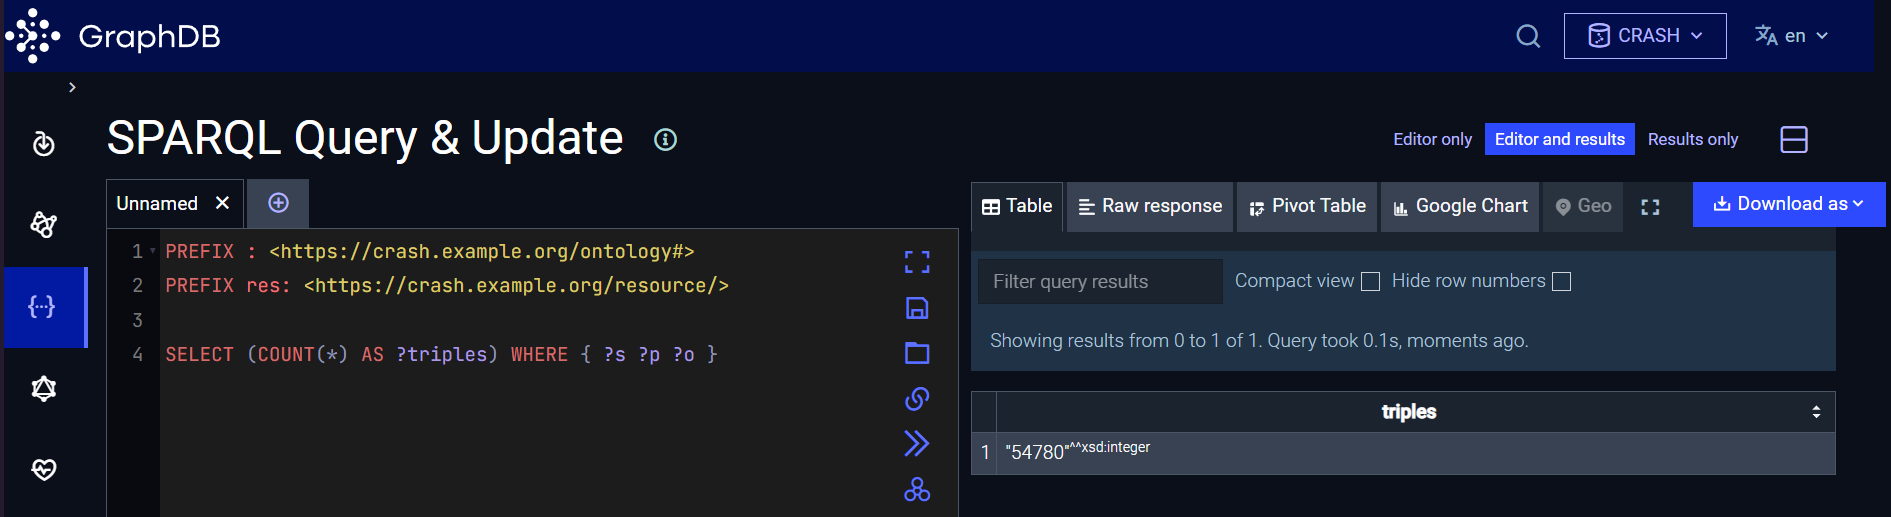
\includegraphics[width=0.7\linewidth]{shot1_triples.png}
\caption{Q1: 54,780 triples in the repository (31,036 explicit plus inferred).}\end{figure}
\begin{figure}[H]\centering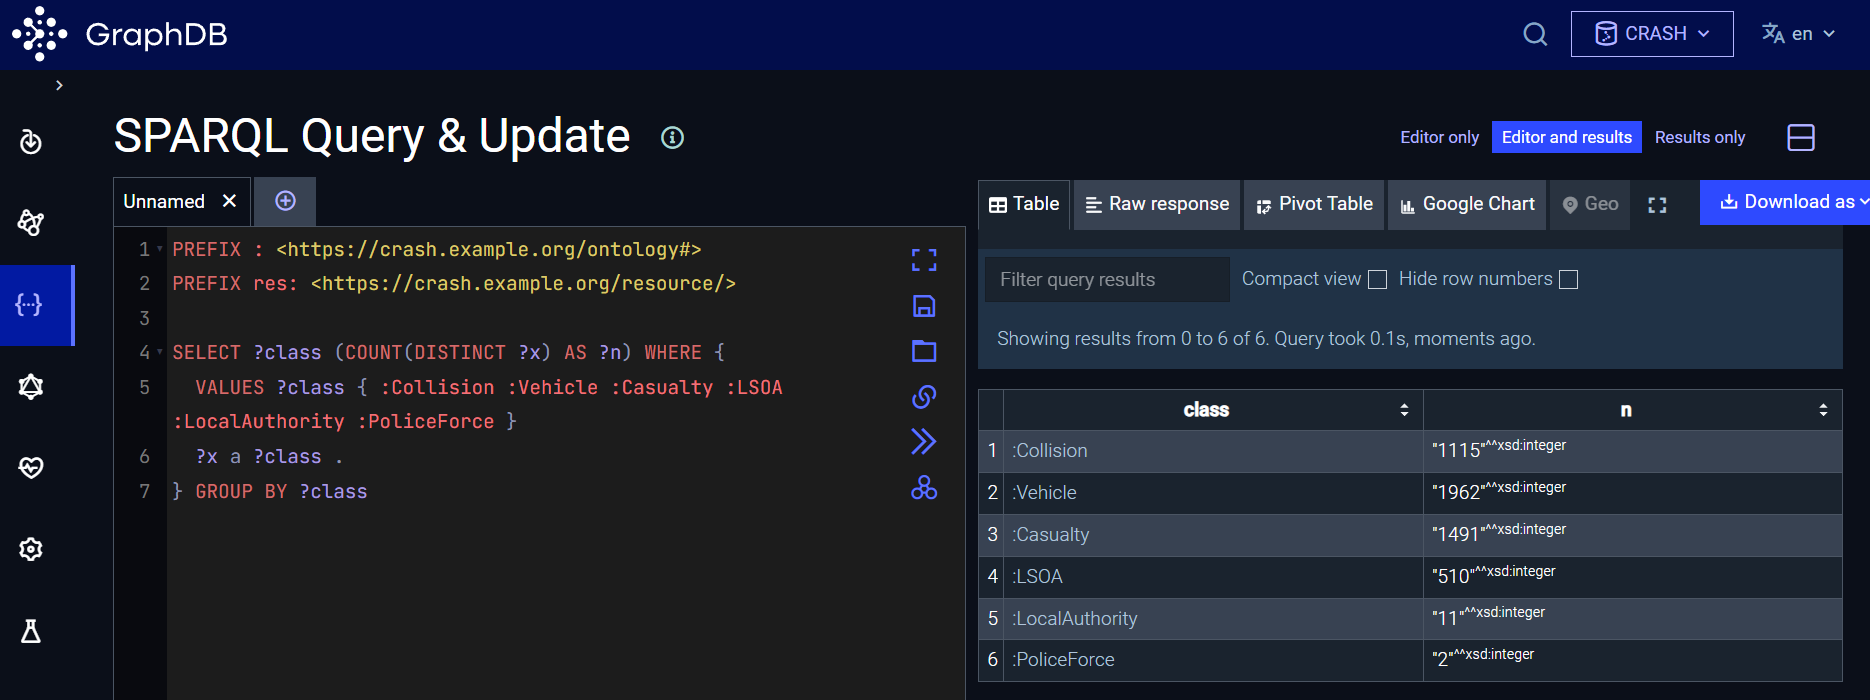
\includegraphics[width=0.7\linewidth]{shot2_classes.png}
\caption{Q2: instances per class match the data file.}\end{figure}
\begin{figure}[H]\centering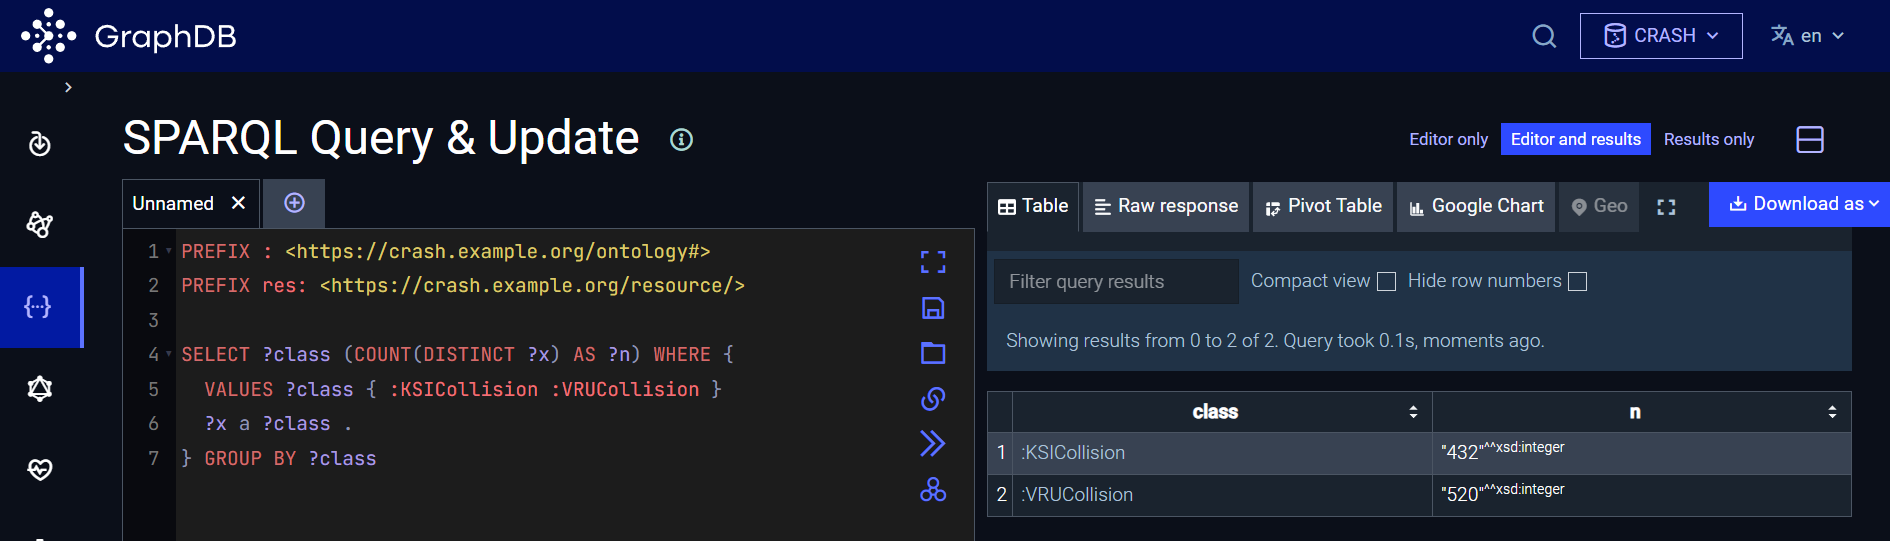
\includegraphics[width=0.7\linewidth]{shot3_inference.png}
\caption{Q3: the reasoner infers 432 KSI collisions and 520 VRU collisions.}\end{figure}
\begin{figure}[H]\centering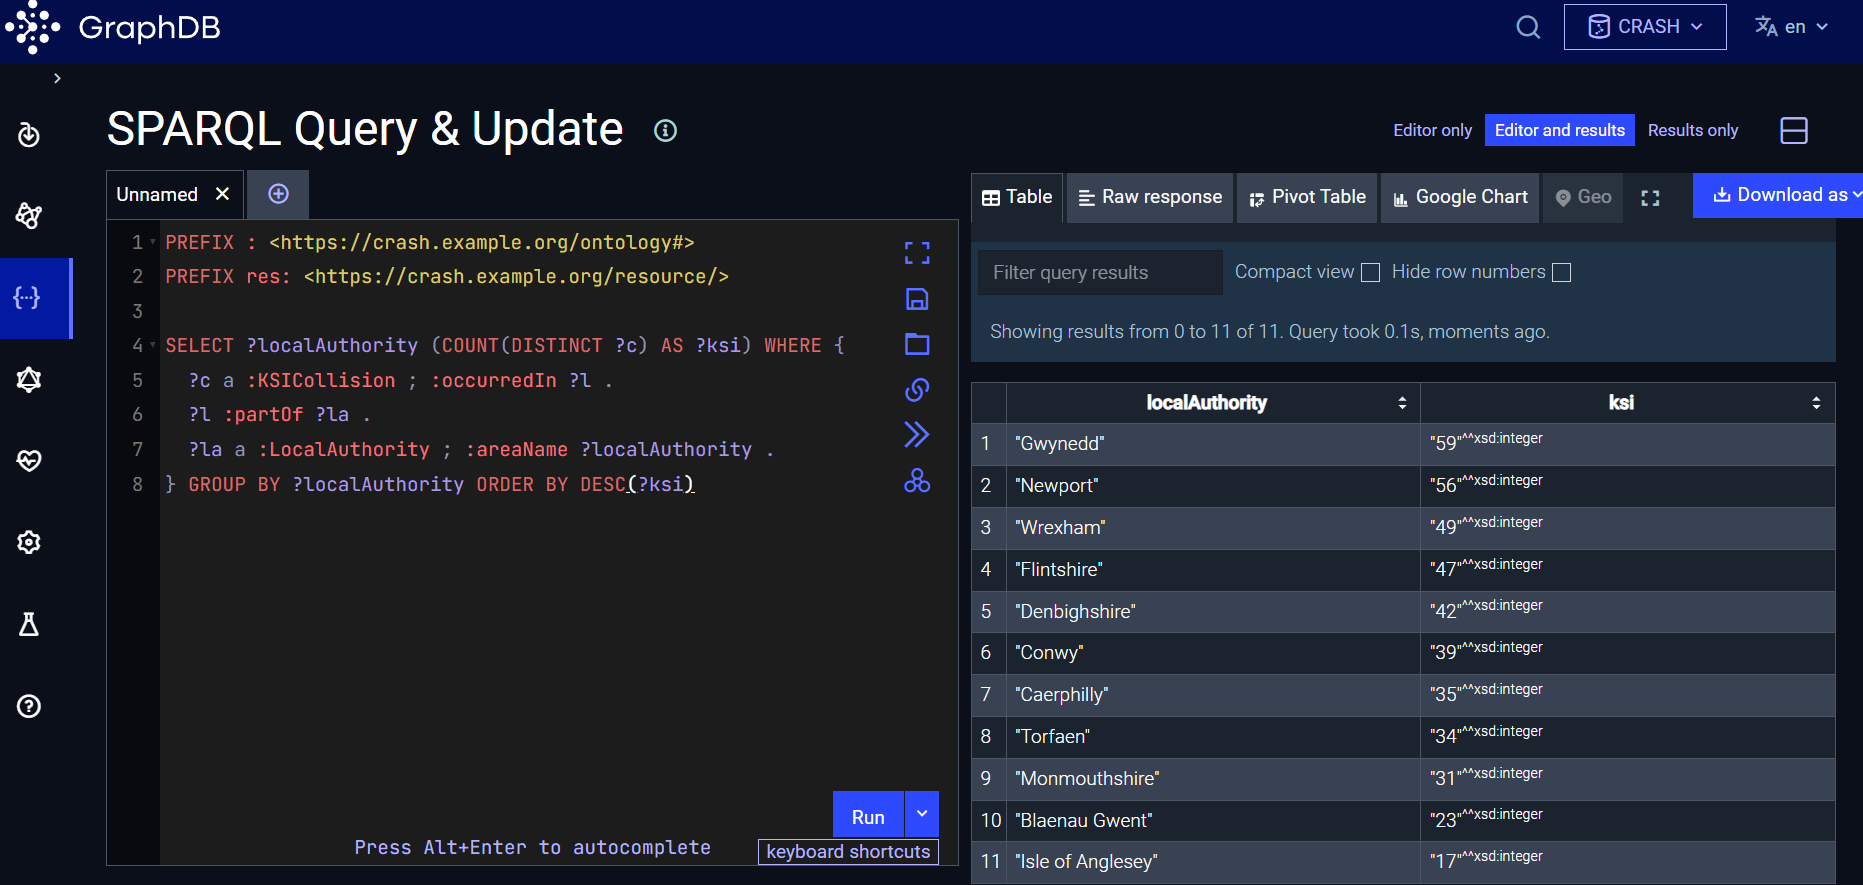
\includegraphics[width=0.7\linewidth]{shot4_ksi_la.png}
\caption{Q4: KSI collisions per local authority (sum 432).}\label{fig:la}\end{figure}
\begin{figure}[H]\centering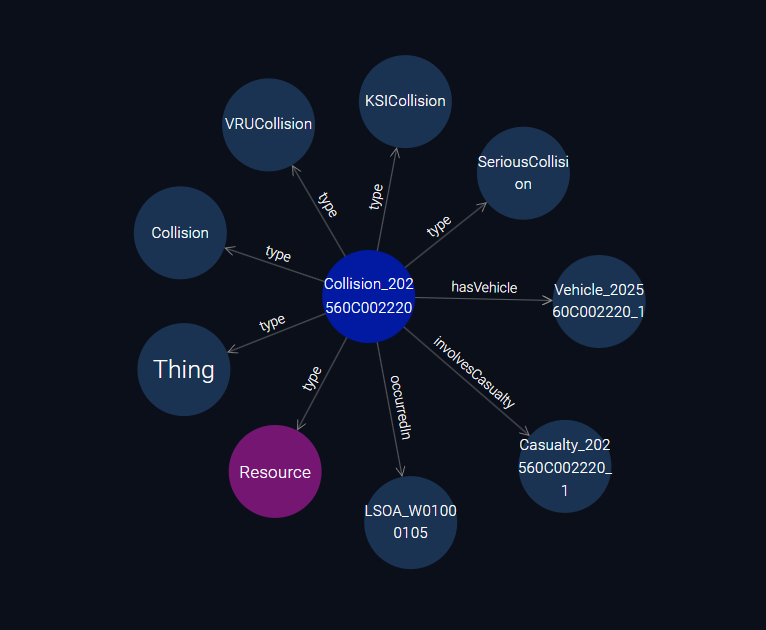
\includegraphics[width=0.42\linewidth]{shot5_visual1.png}
\caption{Q5: Collision\_202560C002220 is stored as SeriousCollision; KSICollision and VRUCollision are inferred. It links to its vehicle, its casualty (\texttt{involvesCasualty}, inferred by a property chain) and LSOA\_W01000105.}\label{fig:v1}\end{figure}
\begin{figure}[H]\centering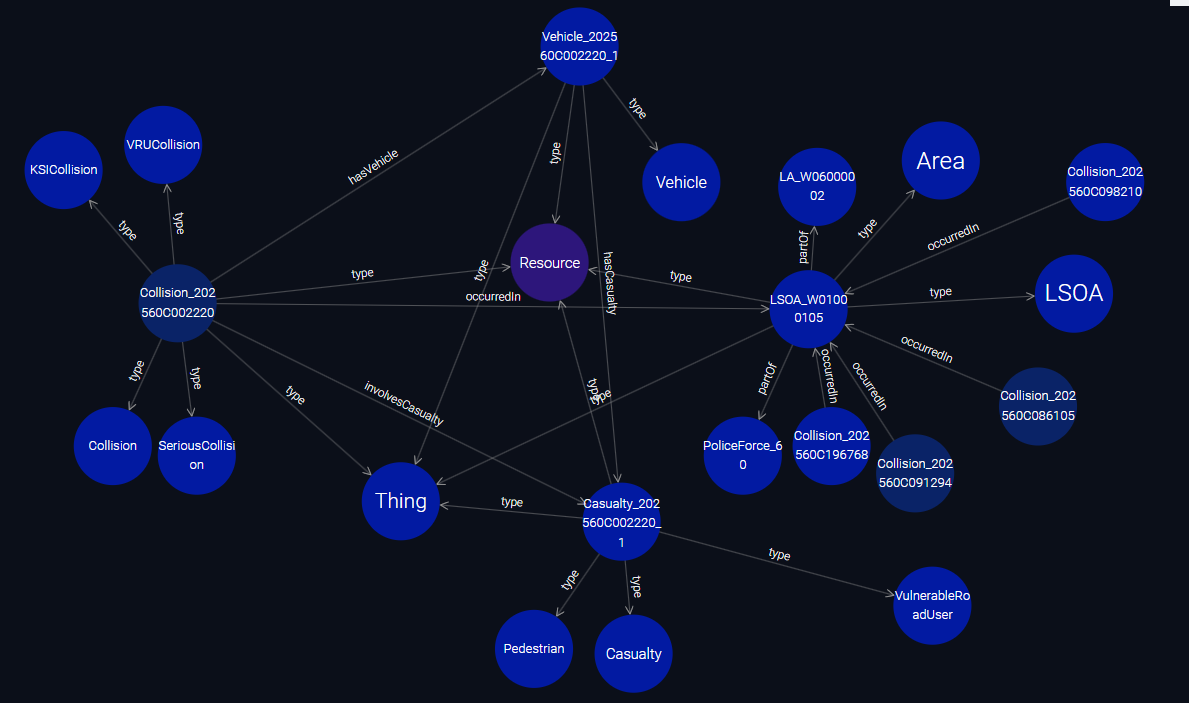
\includegraphics[width=0.75\linewidth]{shot6_visual2.png}
\caption{Q5 expanded: the casualty is a Pedestrian, inferred to be a VulnerableRoadUser; the LSOA is partOf LA\_W06000002 and (by transitivity) PoliceForce\_60.}\label{fig:v2}\end{figure}

\section{Rule-based inference: HighRiskArea}
GraphDB has no SWRL, so rule R7 is run as a SPARQL INSERT: an LSOA with at least 3 KSI collisions becomes a \texttt{HighRiskArea}. The KSI collisions themselves come from the OWL2-RL reasoner. 30 of the 510 LSOAs qualify.
\begin{lstlisting}
# R7 (run once)
INSERT { ?l a :HighRiskArea } WHERE {
  { SELECT ?l WHERE { ?c a :KSICollision ; :occurredIn ?l }
    GROUP BY ?l HAVING (COUNT(DISTINCT ?c) >= 3) } }

# Check: high-risk LSOAs with their local authority and police force
SELECT ?lsoa ?localAuthority ?force (COUNT(DISTINCT ?c) AS ?ksi) WHERE {
  ?l a :HighRiskArea ; :areaCode ?lsoa ; :partOf ?la .
  ?la a :LocalAuthority ; :areaName ?localAuthority ; :partOf ?pf .
  ?pf :areaName ?force .
  ?c a :KSICollision ; :occurredIn ?l .
} GROUP BY ?lsoa ?localAuthority ?force ORDER BY DESC(?ksi) ?lsoa
\end{lstlisting}
\begin{figure}[H]\centering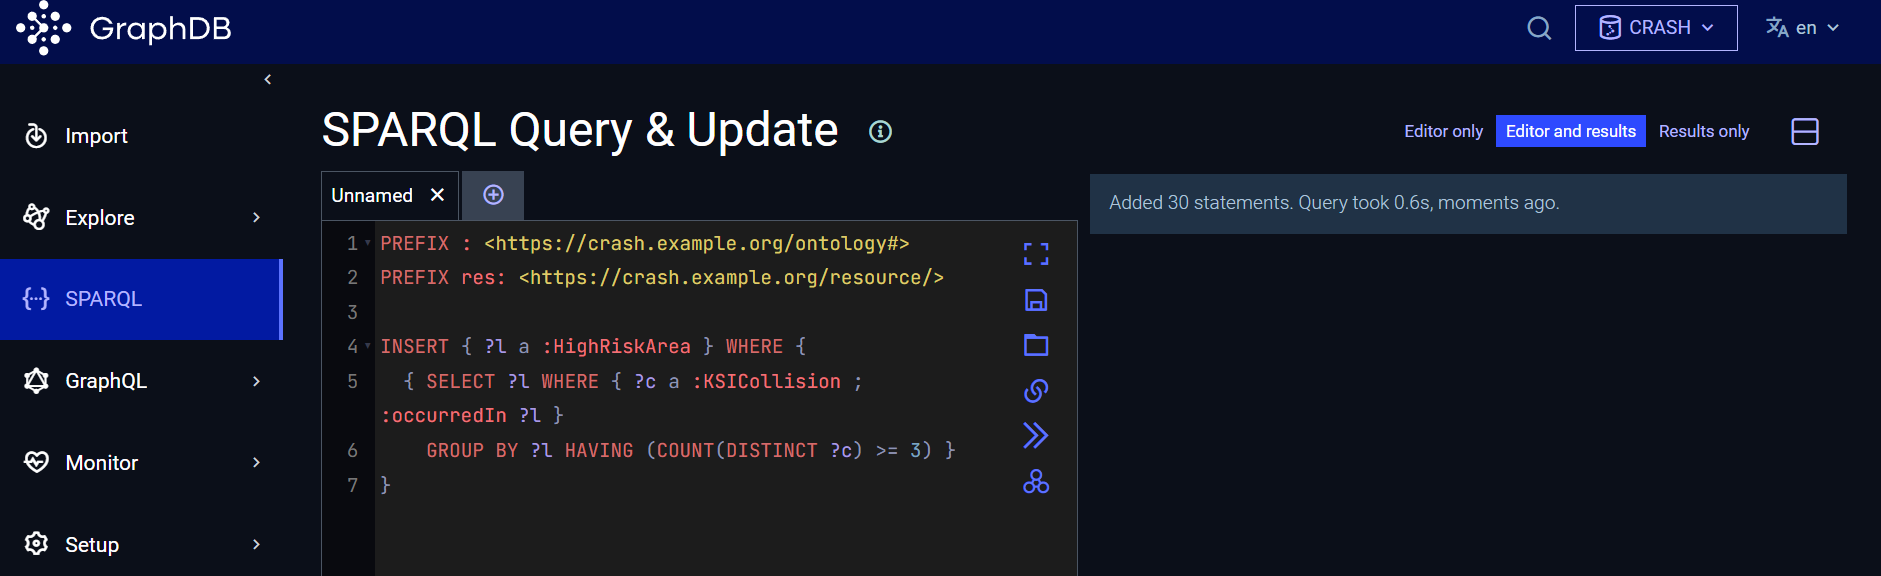
\includegraphics[width=0.7\linewidth]{shot7_r7_insert.png}
\caption{R7: ``Added 30 statements''.}\end{figure}
\begin{figure}[H]\centering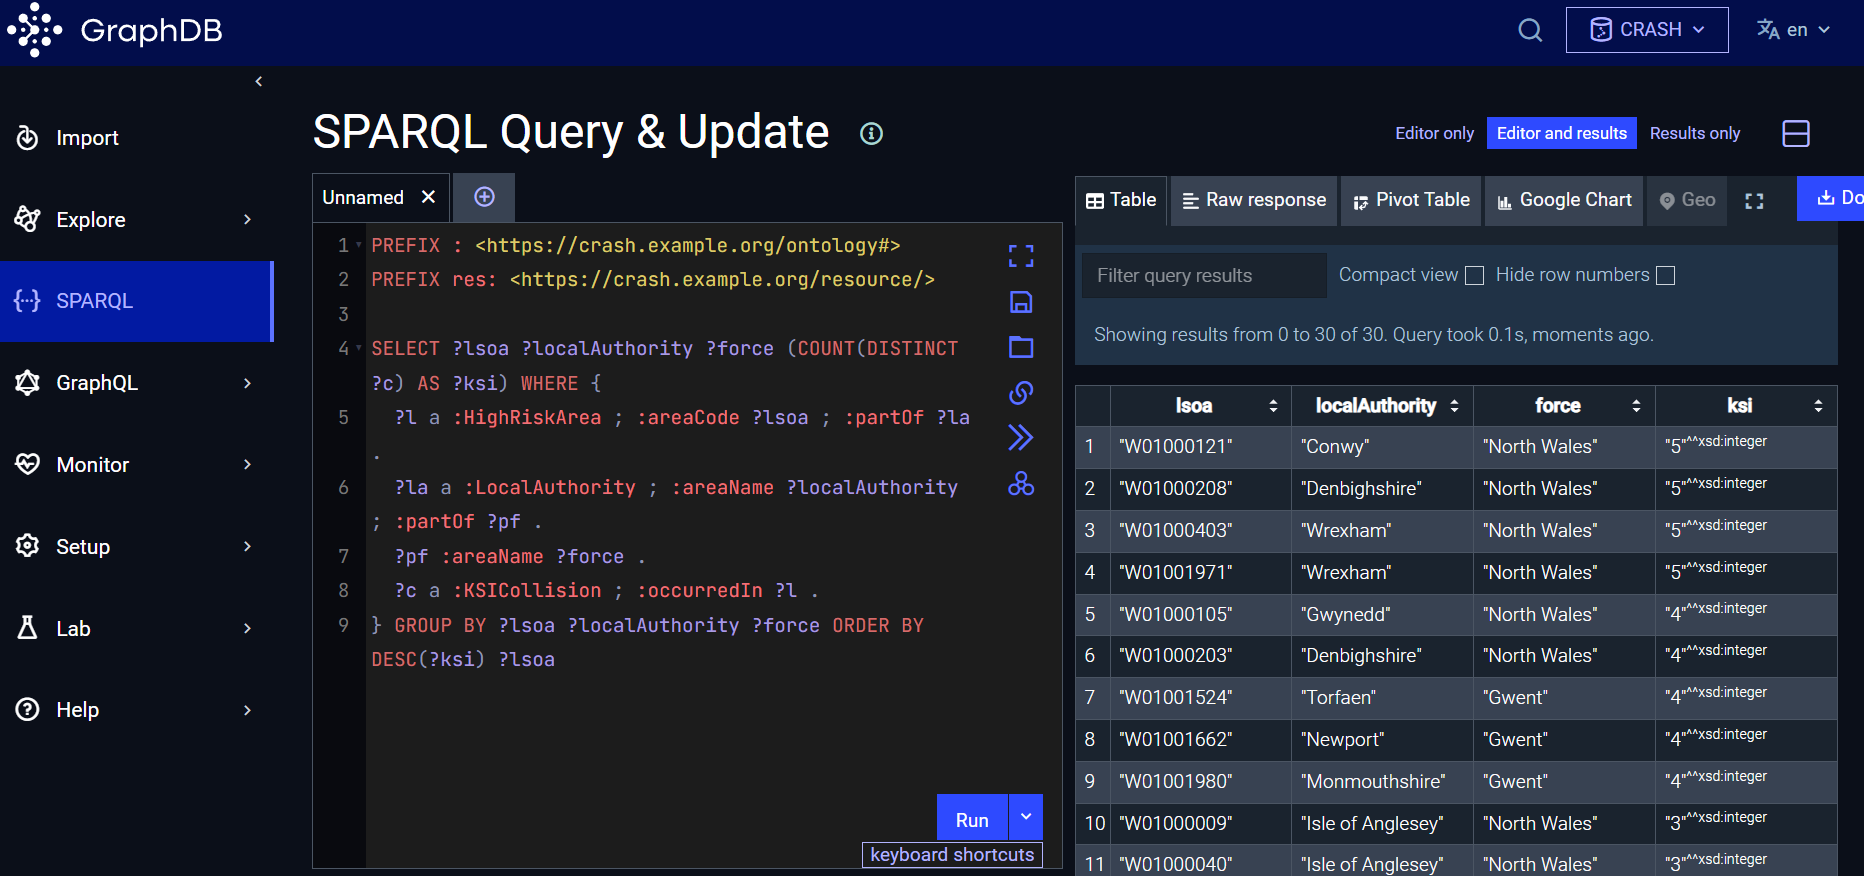
\includegraphics[width=0.7\linewidth]{shot8_r7_check.png}
\caption{Check: 30 high-risk LSOAs (first rows shown), all in North Wales or Gwent, top ones with 5 KSI collisions.}\label{fig:r7}\end{figure}

\section{Conclusion}
The import is verified: every class count in GraphDB matches the data file, and the 11 local-authority counts add up to the 432 KSI collisions. Inference works: \texttt{crash\_data.ttl} stores no \texttt{KSICollision}, \texttt{VRUCollision}, \texttt{VulnerableRoadUser} or \texttt{involvesCasualty} facts, yet GraphDB derives 432 KSI and 520 VRU collisions from the OWL2-RL schema. This explains why the total (54,780) is larger than the 31,036 explicit triples. The HighRiskArea rule (R7) also ran: it classified 30 LSOAs, each traceable to its local authority and police force.
\end{document}
